\documentclass{beamer}
\usetheme{Madrid}

%\usepackage{beamerthemesplit} // Activate for custom appearance

\title[ArchJava]{ArchJava: \newline
Connecting Software Architecture to Implementation}
\subtitle{By Jonathan Aldrich, Craig Chambers, and David Notkin}

\author[Ramya - A05070102]{Presented By: Udaya Ramya Godavarthy}
\institute[TXST]{Texas State University}
\date{\today}
\logo{
\includegraphics[height=1cm]{/Users/godavarthy/Desktop/CS Course Materials/CS5391/Figures/txst_logo.png}}

\begin{document}

\frame{\titlepage}

\section[Outline]{}
\frame{
\frametitle{Table of Contents}
\tableofcontents
}

\section{Precap}
\subsection{Software Architecture}
\frame
{
  \frametitle{Software Architecture}
  \begin{itemize}
  \item Describes the structure of a system 
  \item Enables more effective design, program understanding and formal analysis 
  \item Existing approaches decouple implementation code from architecture 
  \item Leads to inconsistencies, confusion, violation of architectural properties
  \item Inhibits software evolution
  \end{itemize}
}

\frame
{
\frametitle{What is Software Architecture?}
\begin{block}{It is the organization of a software system as a }

  \begin{itemize}
  \item Collection of components \newline
  \item Connections between components \newline
  \item Showing constraints on component interaction \newline
   \end{itemize}
  \end{block}
}

\subsection{Architecture Description Languages (ADL)}
\frame{
\frametitle{Architecture Description Languages (ADL)}
\begin{itemize}
\item Describing architecture in a formal architecture description language (\alert{ADL}) can aid in the specification and analysis of high-level designs. \newline
\item \alert{Limitations: \newline } 
	\begin{itemize}
	\item Existing ADL's are loosely coupled to implementation languages 
	\item Causes problems in analysis, implementation, understanding and evolution of software systems. 
	\newline
	\end{itemize}
\item In summary, while architectural analysis in existing ADLs may reveal important architectural properties but these properties  are not guaranteed to hold in implentation.
\end{itemize}
}

\subsection{Module Interconnection Languages (MIL) }
\frame{
\frametitle{Module Interconnection Languages (MIL)}
\begin{itemize}
\item MILs support system composition from separate modules.
\item ADLs make \alert{connectors} explicit to describe data and control flow between components. 
\item MILs describe the \alert{uses} relationship between modules.
\item MILs cannot be used to describe dynamic architectures, where component object instances are created and linked together at run time.
\item MILs provide encapsulation by hiding names.
\end{itemize}
}

\section{ArchJava Language}
\frame{
\frametitle{ArchJava Language}
\begin{itemize}
\item \alert{ArchJava} is an extension to Java
\item Seamlessly unifies software architectural structure and implementation in one language
\item Allows flexible implementation techniques
\item Ensures traceability between architecture and code
\item Guarantees communication integrity even in presence of advanced architectural features like run time component creation and connection
\item Supports dynamic changes in distributed architectures
\end{itemize}
}

\section{Key Benefits of ArchJava}
\frame{
\frametitle{Key Benefits of ArchJava}
\begin{itemize}
\item include better program understanding \newline
\item reliable architectural reasoning about code \newline
\item keeping architecture and code consistent as they evolve \newline
\item encouraging more developers to take advantage of software evolution \newline
\end{itemize}
}

\section{Language Constructs}
\frame{
\frametitle{Language Constructs}
To allow programmers to describe software architecture, ArchJava adds new language constructs: \newline
\begin{itemize}
\item components \newline
\item connections and \newline
\item ports
\end{itemize}
}

\subsection{Components}
\frame{
\frametitle{Components}
\begin{itemize}
\item A component is a special kind of object that communicates with other components in a structured way.
\item Components communicate at same level through explicitly declared ports 
\item Regular method calls are not allowed
\end{itemize}
}

\subsection{Ports}
\frame{
\frametitle{Ports}
\begin{columns}
\column{0.4 \textwidth}
\begin{itemize}
\item A port represents a logical communication channel between a component and one or more components that it is connected to.
\item Ports declare three sets of methods specified using \alert{requires}, \alert{provides}, and \alert{braodcasts} keywords
\end{itemize}

\column{0.6 \textwidth}
\begin{figure}[htbp]
\begin{center}
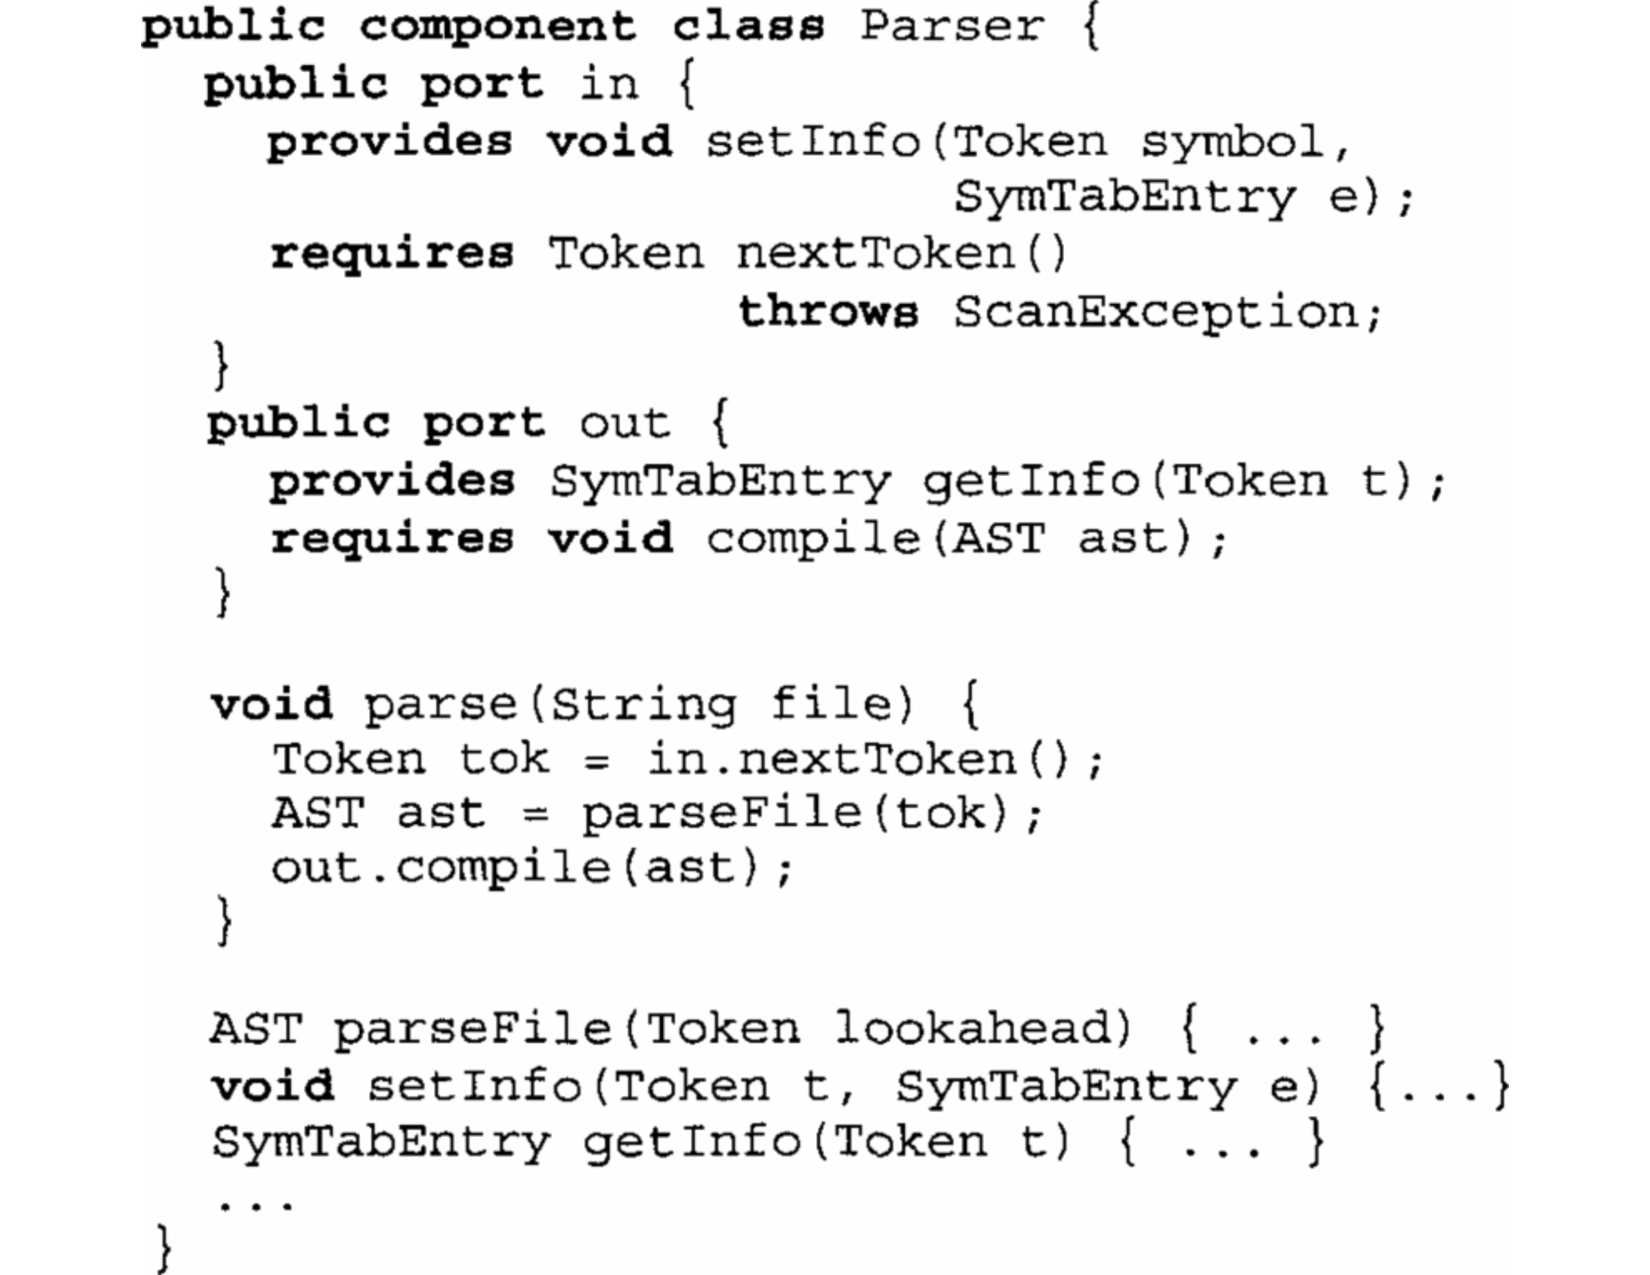
\includegraphics[height=5cm]{/Users/godavarthy/Desktop/CS Course Materials/CS5391/Figures/Figure1.pdf}
\caption{A parser component in ArchJava}
\label{default}
\end{center}
\end{figure}
\end{columns}
}

\subsection{Connections}
\frame{
\frametitle{Connections}
\begin{itemize}
\item Connection consistency checks ensure that each required method is bound to a unique provided method
\item The symmetric connect primitive connects two or more port together, binding each required methods to provided method with the same name and signature.
\item Alternative connection sematics implemented by writing 'smart connector' components 
\end{itemize}
}

\frame{
\frametitle{Compiler Architecture and its ArchJava Representation}
\vspace*{-15mm}
\begin{center}
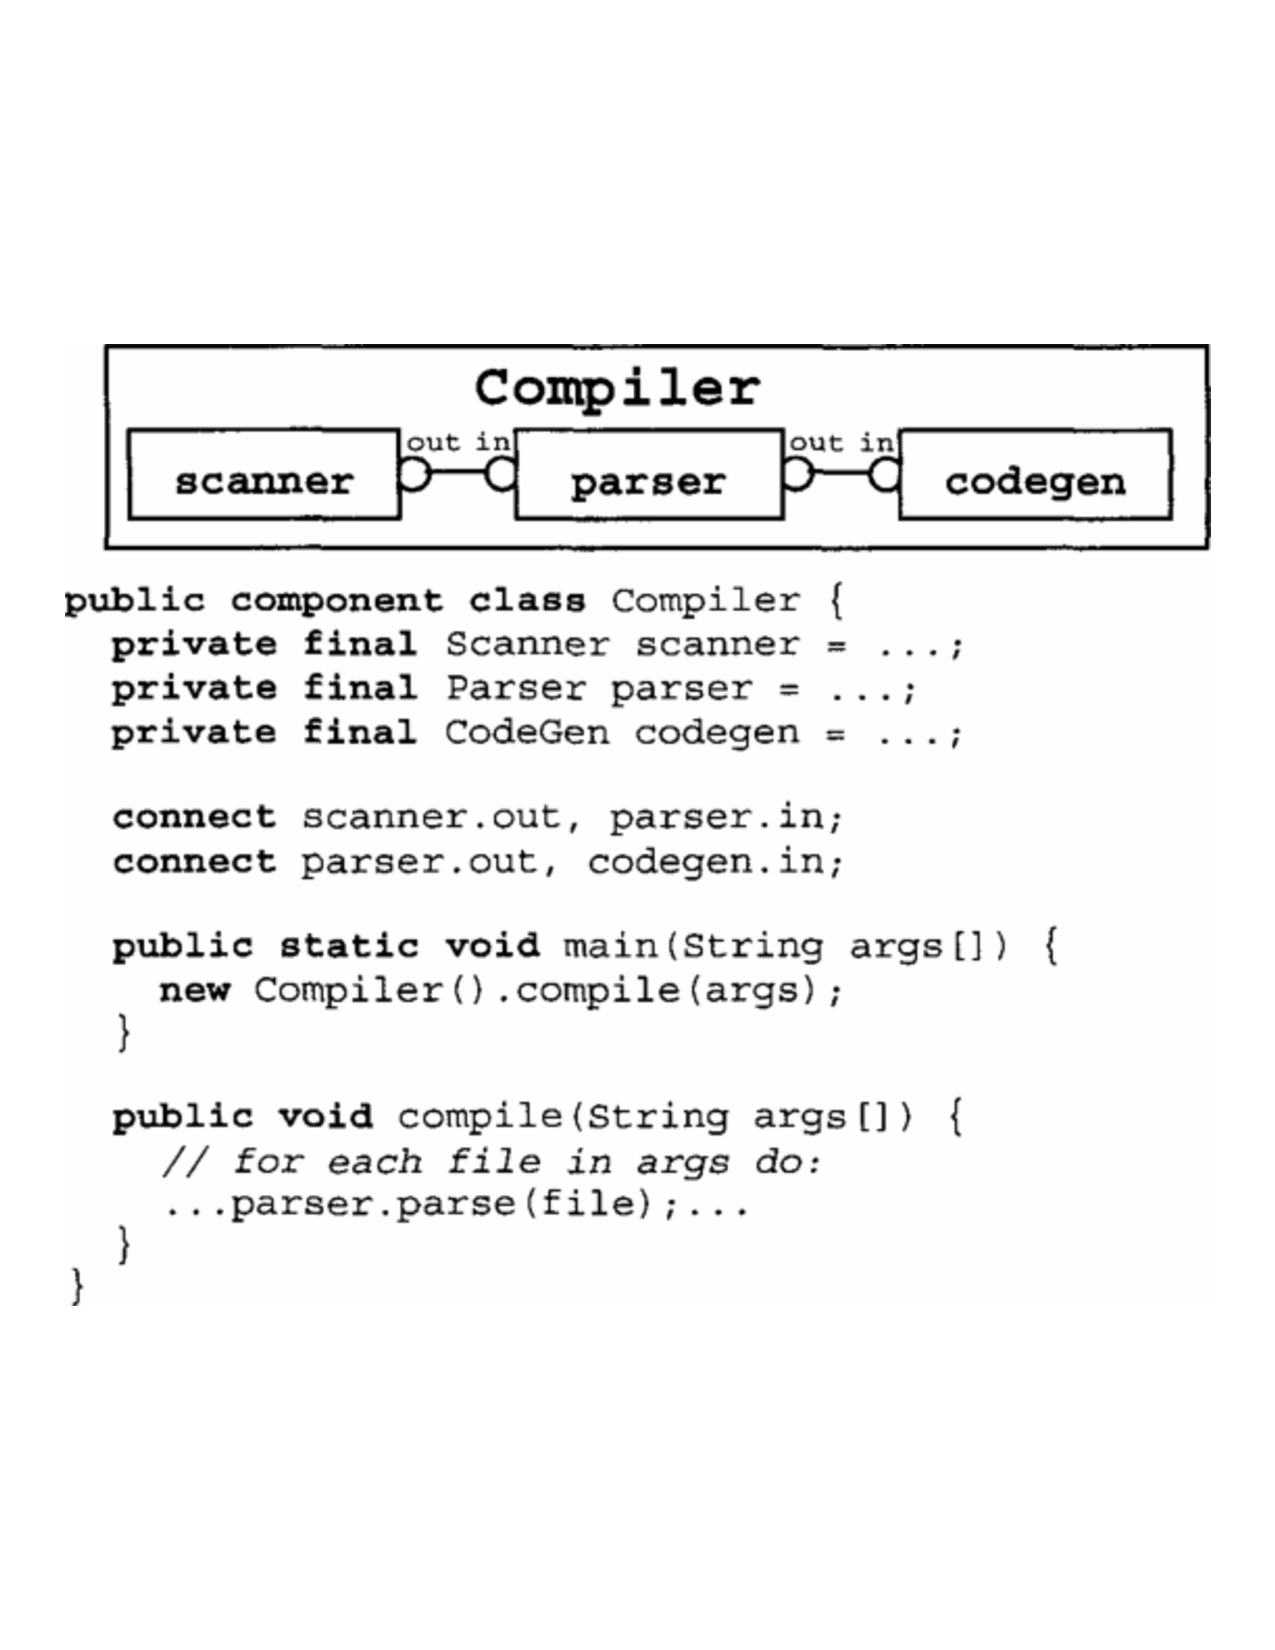
\includegraphics[height=11cm]{/Users/godavarthy/Desktop/CS Course Materials/CS5391/Figures/Figure2.pdf}
\end{center}

}

\frame{
\frametitle{Communication Integrity}
\begin{itemize}
\item Components in an architrecture can only call each other's methods along declared connections between ports.
\item Components are only able to directly invoke methods of their subcomponents.
\end{itemize}
}

\section{Dynamic Architectures}
\frame{
\frametitle{Dynamic Architectures}
\begin{itemize}
\item Covered by creating and connecting together a dynamically determined number of components.
\item Connected using a \alert{connect expression} at run time
\item Each connect expression must match a connection pattern declared in the enclosing component.
\item A \alert{port interface} describes a port that can be instantiated several times to communicate through different connections.
\item Just as Java does not provide a way to explicitly delete objects, ArchJava does not provide a way to explicitly remove components and connections.
\item Components are garbage-collected when they are no longer reachable through direct references or connections.
\end{itemize}
}

\frame{
\frametitle{A Web Server Architecture}
\vspace{-20mm}
\begin{columns}
\column{0.5 \textwidth}
\begin{itemize}
\item Router subcomponent receives incomming HTTP requests and passes them to Worker components that serve the request.
\item The requestWorker method of the web server dynamically creates a Worker component and then connects its serve port to the workers port of the Router.
\end{itemize}

\column{0.6 \textwidth}
\begin{figure}[htbt]
\begin{center}
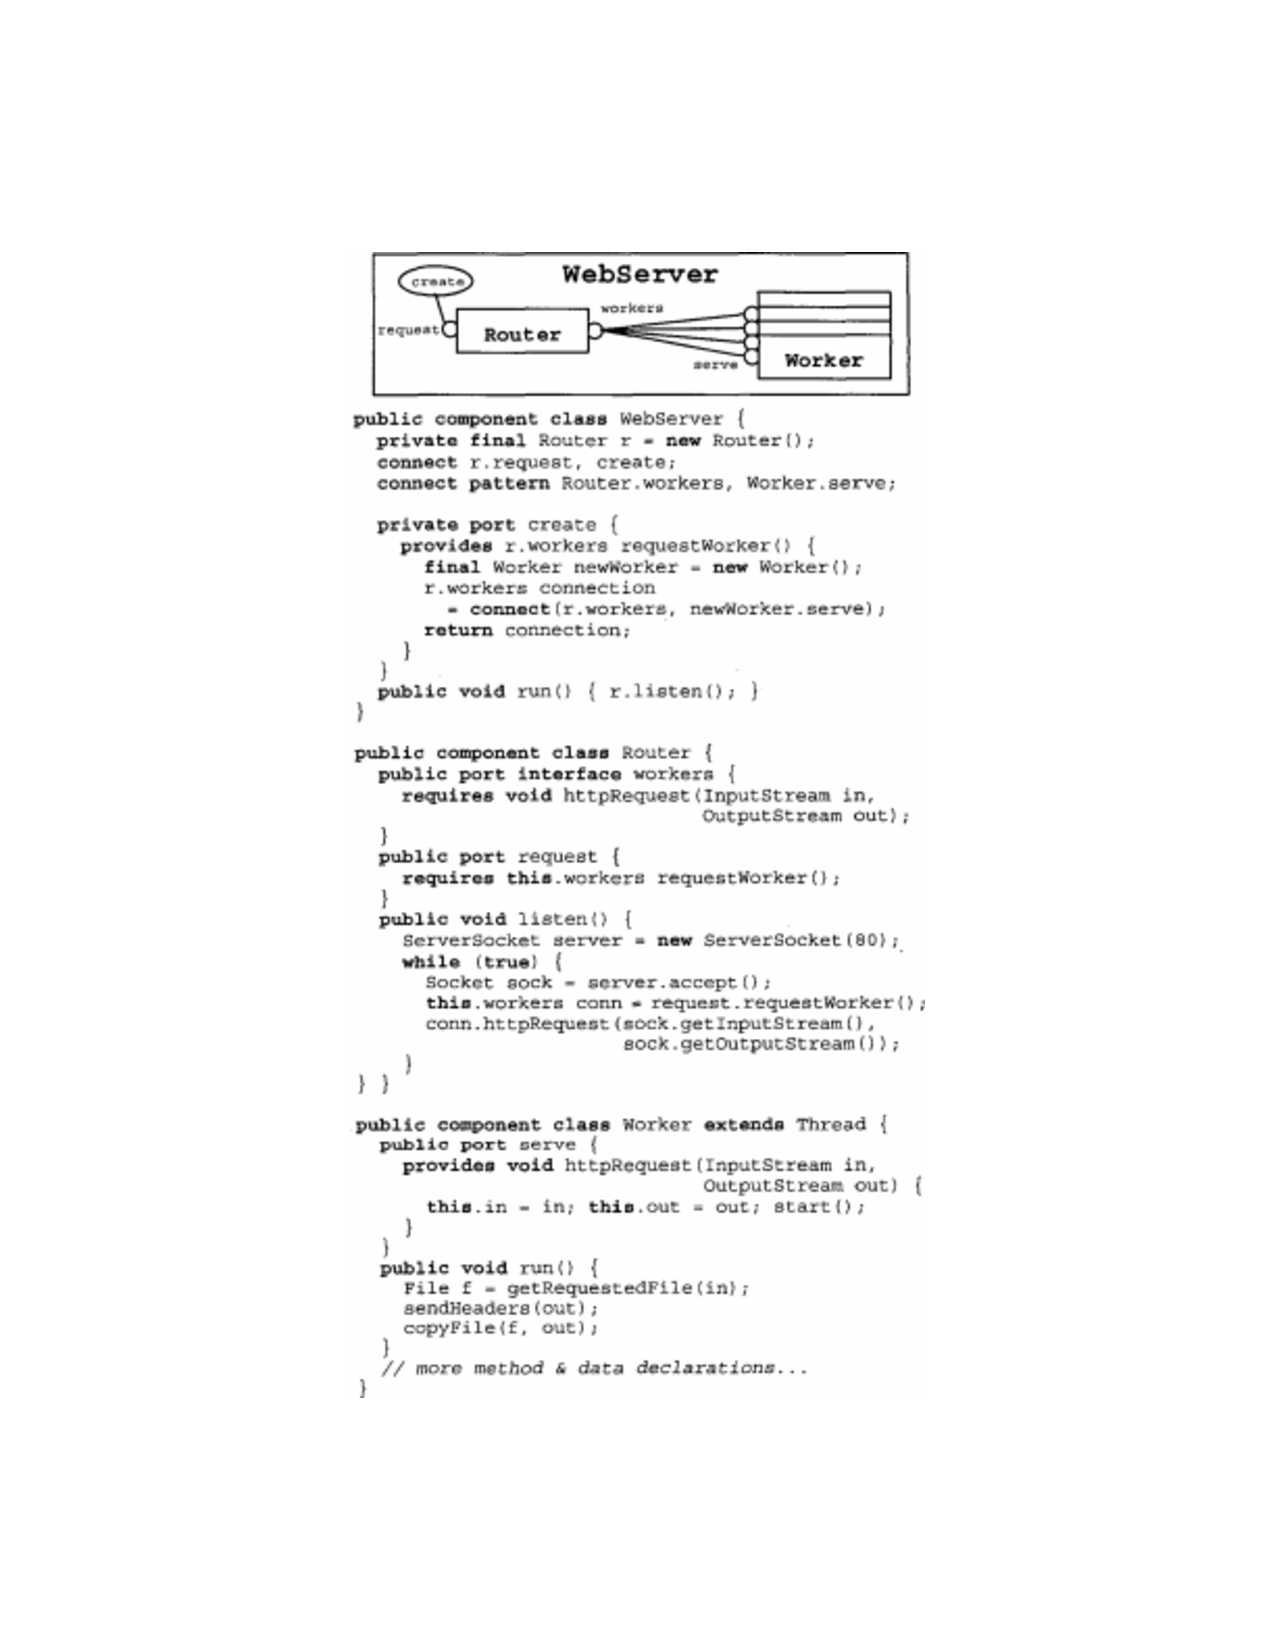
\includegraphics[height=10cm]{/Users/godavarthy/Desktop/CS Course Materials/CS5391/Figures/Figure3.pdf}
\end{center}
\end{figure}

\end{columns}
}

\section{Limitations of ArchJava}
\frame{
\frametitle{Limitations of ArchJava}
\begin{itemize}
\item Only applicable to programs in a single language and running on a single JVM.
\item Architectures in ArchJava are more concrete than architectures in ADLs, restricting the ways in which a given architecture can be implemented.
\item Because of focus on communication integrity, this does not support other architectural reasoning such as connection protocols, architectural styles, or component multiplicity.
\end{itemize}
}

\section{Evaluation}
\frame{
\frametitle{Evaluation}
In order to determine whether the ArchJava language meets its design goals, following questions were addressed: \newline
\begin{enumerate}
\item Can ArchJava express the architecture of a real program of significant complexity?
\item How difficult is it to reengineer a Java program in order to express its architecture explicitly in ArchJava?
\item Does expressing a program’s architecture in ArchJava help or hinder software evolution?
\end{enumerate}
}

\frame{
\frametitle{Hypothesis}
\alert{Hypothesis 1:\newline}

Developers have a conceptual model of their architecture that is mostly accurate, but this model may be a simplification of reality, and it is often not explicit in the code.\newline

\alert{Hypothesis 2: \newline}

Programming languages that prohibit sharing data between components are too inflexible to express the natural architecture for many programs.\newline

}

\frame{
\frametitle{Hypothesis cont'd}
\alert{Hypothesis 3:\newline}

Describing an existing program’s architecture with ArchJava may involve significant restructuring if the desired architecture does not match the implementation well.\newline

\alert{Hypothesis 4: \newline}

Refactoring an application to expose its architecture is done most eficiently in small increments.\newline

\alert{Hypothesis 5:\newline}

Applications can be translated into ArchJava with a modest amount of effort, and without excessive code bloat.\newline

}

\frame{
\frametitle{Hypothesis cont'd}

\alert{Hypothesis 6: \newline}

Expressing software architecture in ArchJava highlights refactoring opportunities by making communication protocols explicit.\newline

\alert{Hypothesis 7:\newline}

Using separate ports and connections to distinguish diflerent protocols and describing protocols with separate provided and required port interfaces may ease program understanding tasks.\newline

}

\frame{
\frametitle{Hypothesis cont'd}

\alert{Hypothesis 8: \newline}

Communication integrity in ArchJava encourages local communication and helps to reduce coupling between components.\newline

\alert{Hypothesis 9: \newline}

An explicit sofiware architecture makes it easier to identify and evolve the components involved in a change.\newline

}

\frame{
\frametitle{Aphyds Architecture}
\begin{figure}[htbt]
\begin{center}
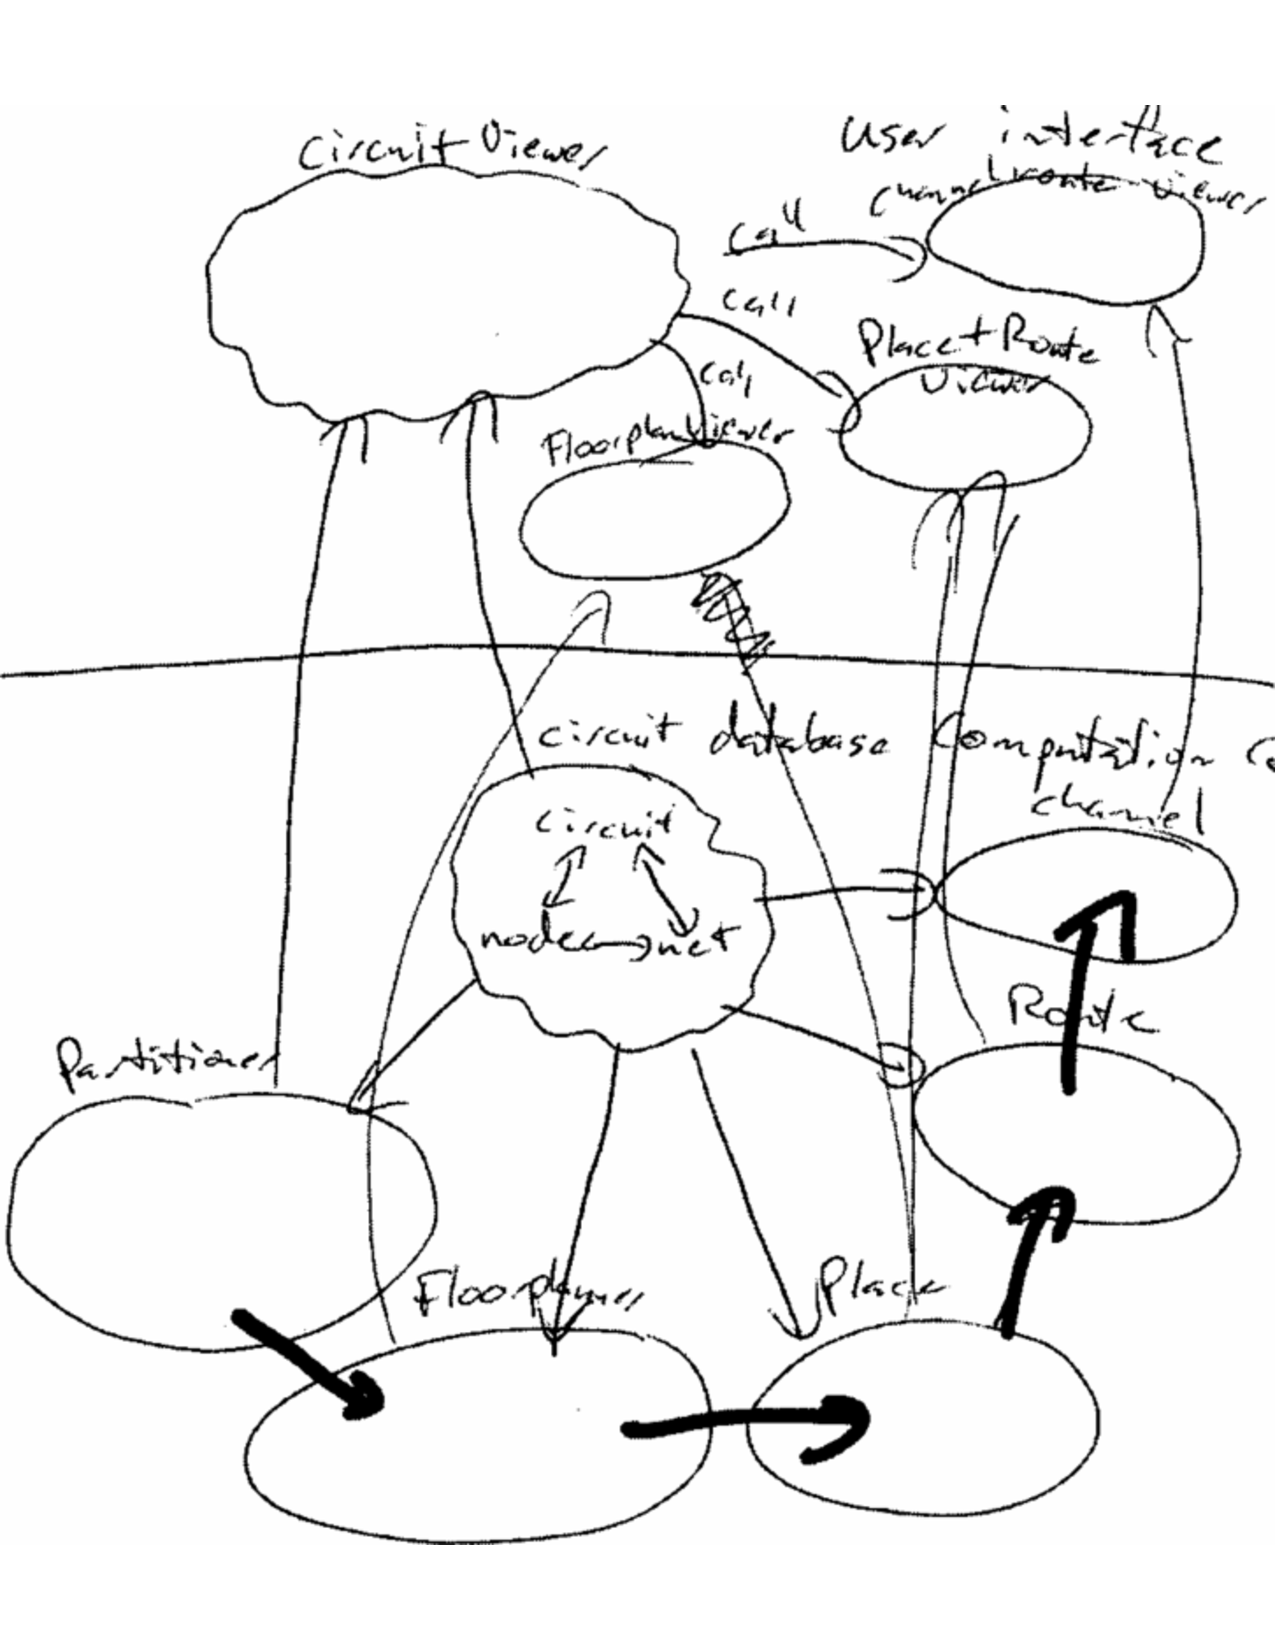
\includegraphics[height=8cm]{/Users/godavarthy/Desktop/CS Course Materials/CS5391/Figures/Figure4.pdf}
\end{center}
\end{figure}
}

\frame{
\frametitle{Aphyds Architecture cont'd}
\vspace{-30mm}
\begin{figure}[htbt]
\begin{center}
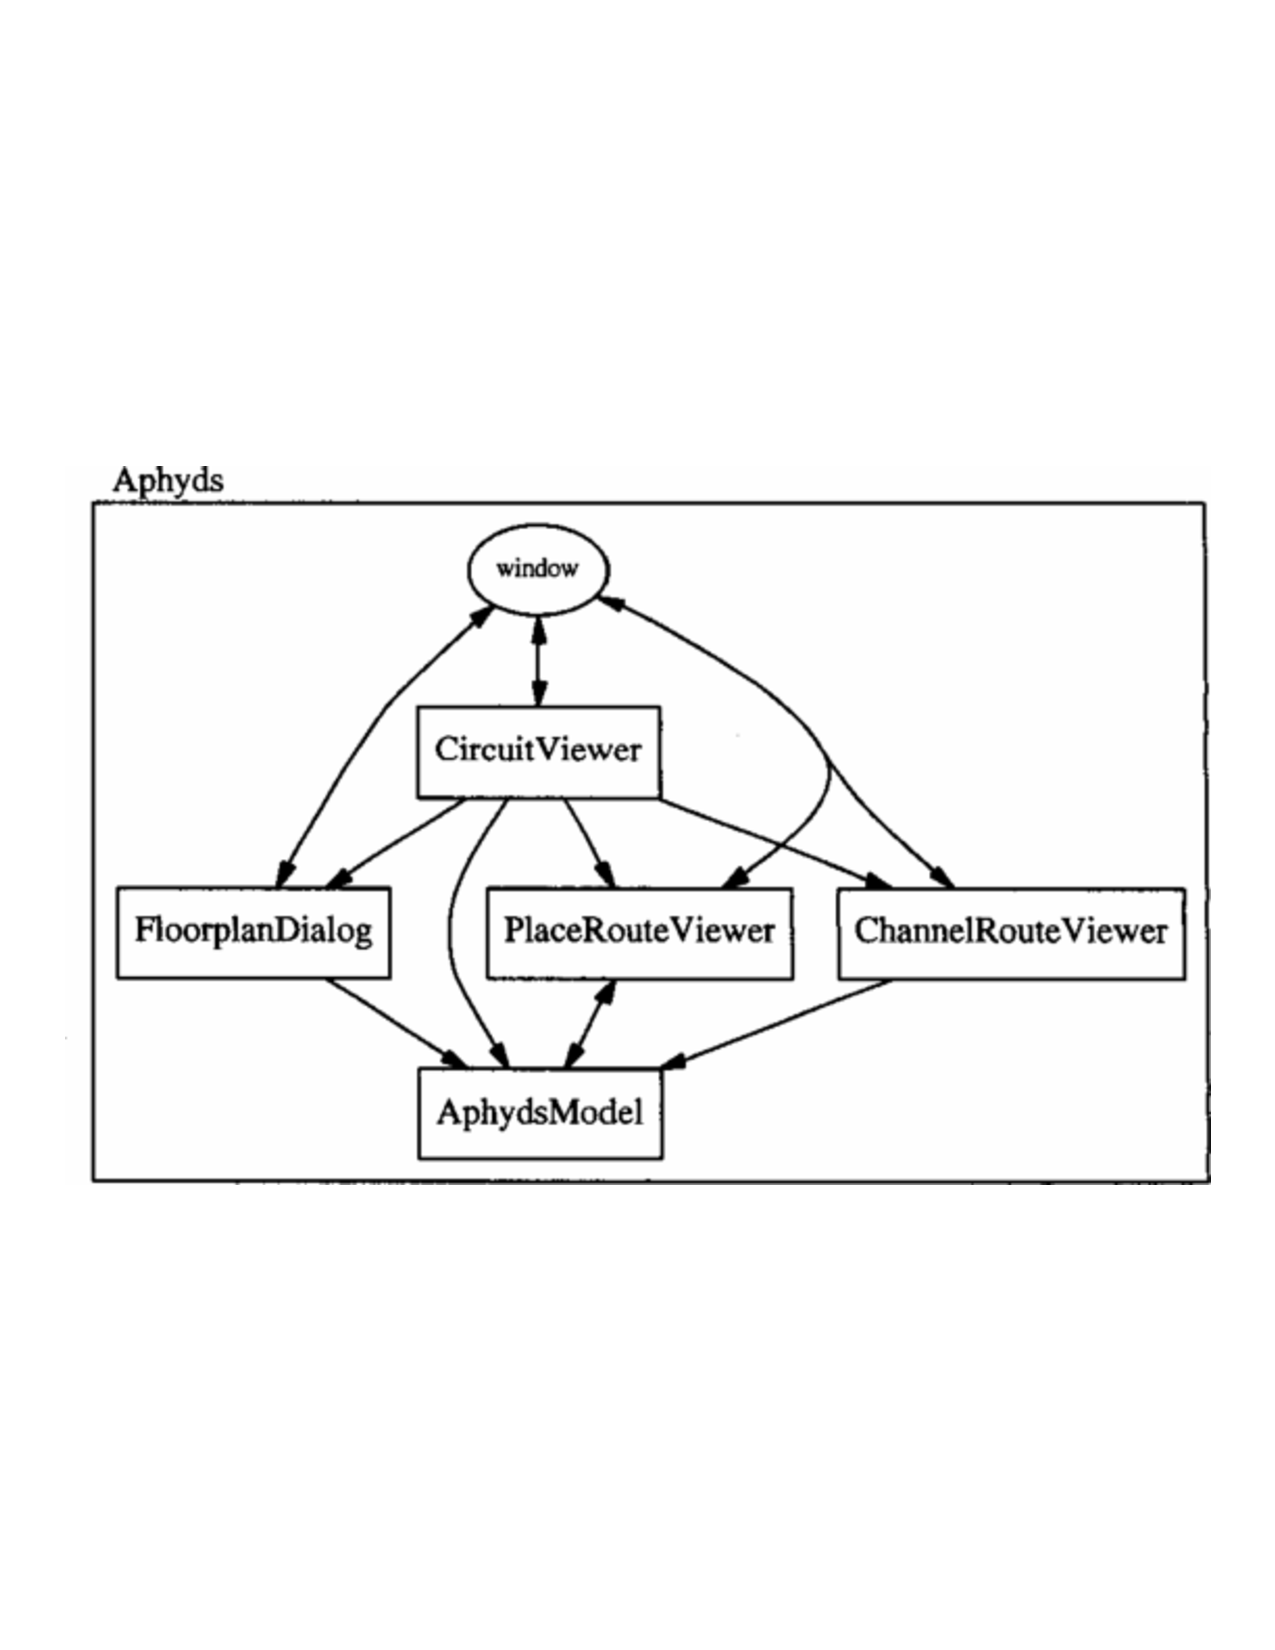
\includegraphics[height=13cm]{/Users/godavarthy/Desktop/CS Course Materials/CS5391/Figures/Figure6.pdf}
\end{center}
\end{figure}
}

\frame{
\frametitle{References}
\centering
\begin{thebibliography}
\bibitem{} Aldrich, Jonathan, Craig Chambers, and David Notkin.  \textquotedblleft ArchJava: Connecting software architecture to implementation.\textquotedblright\ \textit{Proceedings of the 24th International Conference on Software Engineering}. ICSE 2002. IEEE, 2002.
\end{thebibliography}
}
\end{document}
